\documentclass{article}

% Geometry package
\usepackage[a4paper, margin=1in]{geometry}

% Math packages
\usepackage{amsmath}
\usepackage{amssymb}
\usepackage{amsthm}

% Other packages
\usepackage{hyperref}
\usepackage{float}

% Graphics
\usepackage{graphicx}
\usepackage{tikz}
\usetikzlibrary{shapes, arrows}

% Code
\usepackage{listings}
\usepackage{xcolor}

\lstdefinestyle{SystemVerilogStyle}{
    language=Verilog,
    basicstyle=\small\ttfamily,
    keywordstyle=\color{blue}\bfseries,
    commentstyle=\color{green!60!black},
    morecomment=[l]{//},
    morecomment=[s]{/*}{*/},
    stringstyle=\color{orange},
    breaklines=true,
    showstringspaces=false,
    numbers=left,
    numberstyle=\tiny,
    numbersep=5pt,
    backgroundcolor=\color{gray!10},
    frame=single,
    rulecolor=\color{black!40},
    captionpos=b,
    tabsize=4,
    morekeywords={module, endmodule, input, output, reg, always, begin, end, if,
    else, for, while, case, endcase, logic, $dumpvars, $dumpfile}
}

% Title
\renewcommand{\maketitle}{
  \begin{flushleft}
    ZC - University of Science and Technology
    \hfill Fall 2023 \\
    Communications \& Information Engineering Program \\
    CIE 239: Digital Design and Computer Architecture
  \end{flushleft}
  \begin{center}
    \Huge Digital Arithmetic and Logic Unit \\
    \Large \textit{Project Overview}
  \end{center}
  \begin{flushleft}
    Team Members: \\

    \begin{tabular}{ccc}
      202200341 & Abdulrahman Magdy & \href{mailto:s-abdulrahman.abdulrahman@zewailcity.edu.eg}{s-abdulrahman.abdulrahman@zewailcity.edu.eg} \\
      202201079 & SalahDin Rezk & \href{mailto:s-salahdin.rezk@zewailcity.edu.eg}{s-salahdin.rezk@zewailcity.edu.eg} \\
      202200285 & Shehab Mohamed & \href{mailto:s-shehab.mohamed@zewailcity.edu.eg}{s-shehab.mohamed@zewailcity.edu.eg} \\
    \end{tabular}  \\
  \end{flushleft}
}

% Document
\begin{document}

% front matter
\maketitle
\tableofcontents
\listoffigures
\listoftables

\begin{abstract}
  The Digital Arithmetic Logic Unit (ALU) is a crucial component in digital
  systems, responsible for performing arithmetic and logical operations. This
  project focuses on designing and implementing a 4-bit ALU using System Verilog.
  The ALU will be capable of handling basic arithmetic operations such as
  addition and subtraction, as well as logical operations like AND, OR, and
  XOR.
\end{abstract}

% main matter
\section{Design}

\subsection{Requirements}

\begin{table}[H]
  \caption{ALU Operations}
  \begin{center}
    \begin{tabular}[c]{l|l}
      \hline
      \multicolumn{1}{c|}{\textbf{Operation}} & 
      \multicolumn{1}{c}{\textbf{Output (E)}} \\
      \hline
      OR & $E = A \lor B$ \\
      AND & $E = A \land B$ \\
      CMP & $E = \overline{B} $ \\
      ADD & $E = A + B$ \\
      SUB & $E = A - B$ \\
      XOR & $E = A \oplus B$ \\
      ASR & $E_{3:0}=A_{3}A_{2}A_{1}A_{0}$ \\
      INC & $E = B + 1$ \\
      \hline
    \end{tabular}
  \end{center}
\end{table}

\begin{table}[H]
  \begin{minipage}{.5\linewidth}
    \centering
    \caption{ALU Inputs}
    \begin{tabular}{l|l}
      \hline
      \textbf{Inputs} & \textbf{Description} \\
      \hline
      $A_{3:0}$ & First operand \\
      $B_{3:0}$ & Second operand \\
      $C_{in}$ & Carry-in \\
      $S_{2:0}$ & Operation selection \\
      \hline
    \end{tabular}
  \end{minipage}%
  \begin{minipage}{.5\linewidth}
    \centering
    \caption{ALU Outputs}
    \begin{tabular}{l|l}
      \hline
      \textbf{Output} & \textbf{Description} \\
      \hline
      $E_{3:0}$ & Result \\
      $C_{out}$ & Carry-out \\
      $Z$ & Zero output \\
      $V$ & Overflow \\
      \hline
    \end{tabular}
  \end{minipage}
\end{table}

\subsection{Structure}

The project is structured into two main components: the Arithmetic Unit and the
Logic Unit. Inputs \(A\) and \(B\) both are 4-bit signals while selection \(S\)
is 3-bit and \(C_{in}\) is one-bit. The output \(E\) is 4-bit while \(C_{out}\),
\(Z\), and \(V\) are one-bit. Both units are connected to the same input and
output signals. Figure \ref{fig:ALU_flowchart} shows the flowchart of the ALU
structure, while Figure \ref{fig:ALU_structure} shows the schematic of the
structure. Finally, Table \ref{tab:ALU_selection} shows the Mux configuration
for the ALU selection.

\begin{figure}[H]
  \centering
  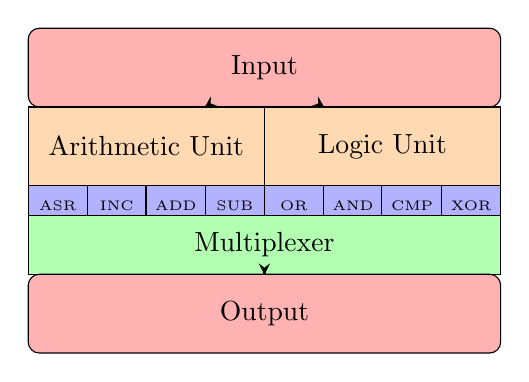
\begin{tikzpicture}
    % Define styles
    \tikzstyle{startstop} = [rectangle, rounded corners, minimum width=6cm, minimum height=1cm, text centered, draw=black, fill=red!30]
    \tikzstyle{process} = [rectangle, minimum width=3cm, minimum height=1cm, text centered, draw=black, fill=orange!30]
    \tikzstyle{operation} = [rectangle, minimum width=0.75cm, minimum height=0.5cm, text centered, draw=black, fill=blue!30]
    \tikzstyle{arrow} = [thick,->,>=stealth]

    % Nodes
    \node (start) [startstop] {Input};
    \node (arith) [process, below of=start, xshift=-1.5cm] {Arithmetic Unit};
    \node (ASR) [operation, below of=arith, yshift=0.25cm, xshift=-1.125cm] {\tiny ASR};
    \node (INC) [operation, below of=arith, yshift=0.25cm, xshift=-0.375cm] {\tiny INC};
    \node (ADD) [operation, below of=arith, yshift=0.25cm, xshift=0.375cm] {\tiny ADD};
    \node (SUB) [operation, below of=arith, yshift=0.25cm, xshift=1.125cm] {\tiny SUB};
    \node (logic) [process, below of=start, xshift=1.5cm] {Logic Unit};
    \node (OR) [operation, below of=logic, yshift=0.25cm, xshift=-1.125cm] {\tiny OR};
    \node (AND) [operation, below of=logic, yshift=0.25cm, xshift=-0.375cm] {\tiny AND};
    \node (CMP) [operation, below of=logic, yshift=0.25cm, xshift=0.375cm] {\tiny CMP};
    \node (XOR) [operation, below of=logic, yshift=0.25cm, xshift=1.125cm] {\tiny XOR};
    \node (mux) [process, below of=arith, minimum width=6cm, yshift=-0.25cm, xshift=1.5cm, minimum height=0.75cm, fill=green!30] {Multiplexer};
    \node (end) [startstop, below of=arith, xshift=1.5cm, yshift=-1.125cm] {Output};
    
    % Arrows
    \draw [arrow] (arith) -- (start);
    \draw [arrow] (logic) -- (start);
    \draw [arrow] (end) -- (mux);
  \end{tikzpicture}
  \caption{ALU Structure Flowchart}\label{fig:ALU_flowchart}
\end{figure}

\begin{figure}[htpb]
  \begin{center}
    \includegraphics[width=\textwidth]{figures/ALU_structure.pdf}
  \end{center}
  \caption{ALU Structure Diagram}\label{fig:ALU_structure}
\end{figure}

\begin{table}[htpb]
  \caption{MUX Configurations for ALU Selection}\label{tab:ALU_selection}
  \begin{center}
    \begin{tabular}{c|c}
      \hline
      \( s_{2} \) & Operation \\
      \hline
      0 & Arithmetic Unit \\
      1 & Logic Unit \\
      \hline
    \end{tabular}
  \end{center}
\end{table}


\subsection{Arithmetic Unit}

\begin{enumerate}
  \item Input Signals
    \begin{itemize}
      \item The Arithmetic Unit receives two 4-bit inputs, \(A\) and \(B\) in
        the form of two's complement numbers.
      \item The reason behind using two's complement is that it allows for
        addition and subtraction to be performed using the same circuitry.
    \end{itemize}
  \item 4-Bit Operations
    \begin{itemize}
      \item The Arithmetic Unit comprises four Full Adders and 4x1 MUXs for
        versatile 4-bit operations. 
      \item The first set of MUXs facilitates selection among operations,
        including ASR, Increment, addition, or subtraction. 
    \end{itemize}
  \item MUX Configurations
    \begin{itemize}
      \item Four inputs to the first MUXs correspond to:
        \begin{table}[H]
          \caption{MUX Configurations for Arithmetic Unit}
          \begin{center}
            \begin{tabular}{c|c|c}
              \hline
              \( S_{0} \) & \( C_{in} \) & Operation \\
              \hline
              0 & 0 & ASR \\
              0 & 1 & $A - B$ \\
              1 & 0 & $A + B$ \\
              1 & 1 & $B + 1$ \\
              \hline
            \end{tabular}
          \end{center}
        \end{table}
      \item Another set of MUXs manage the shift of A or set A to 0 for incrementing B. 
    \end{itemize}
  \item Bitwise Calculations
    \begin{itemize}
      \item Each bit of the output is computed using a Full Adder and two MUXs. 
      \item The Full Adder generates two outputs: the corresponding bit of E
        and the carry-out, which serves as the carry-in for the subsequent Full
        Adder. 
    \end{itemize}
  \item Overflow Detection
    \begin{itemize}
      \item Overflow is detected by comparing the sign bits of A and B, and
        comparing the sign bit of E.
        \begin{align*}
          V = \overline{A_{3}}\,\overline{B_{3}} E_{3} + A_{3}B_{3}\overline{E_{3}}
        .\end{align*}
        Generating the following truth table:
        \begin{table}[H]
          \begin{center}
            \begin{tabular}{c|c|c|c}
              \hline
              $A_{3}$ & $B_{3}$ & $E_{3}$ & $V$ \\
              \hline
              0 & 0 & 0 & 0 \\
              0 & 0 & 1 & 1 \\
              0 & 1 & 0 & 0 \\
              0 & 1 & 1 & 0 \\
              1 & 0 & 0 & 0 \\
              1 & 0 & 1 & 0 \\
              1 & 1 & 0 & 1 \\
              1 & 1 & 1 & 0 \\
              \hline
            \end{tabular}
          \end{center}
        \end{table}
        Which is equivalent to XOR of (A, B) and E.
      \item The rationale behind this decision is that overflow occurs when the
        sign bits of A and B are the same, but the sign bit of E is different.
        That is a result of adding two positive numbers and getting a negative
        number, or adding two negative numbers and getting a positive number in
        the two’s complement system.
    \end{itemize}
  \item Zero Output Determination
    \begin{itemize}
      \item Output $Z$ is determined using a NOR gate, signaling 1 only if all
        inputs are zeros. 
        \begin{align*}
          Z =
          \overline{E_{3}}\,\overline{E_{2}}\,\overline{E_{1}}\,\overline{E_{0}}
        .\end{align*}
    \end{itemize}
\end{enumerate}

\subsection{Logic Unit}
\begin{enumerate}
  \item Operation Selection: 
    \begin{itemize}
      \item The Logic Unit utilizes the least significant bits of S to decide
        between AND, OR, inversion, or XOR operations on A and B. Multiplexers
        are used to select the appropriate operation.
        \begin{table}[htpb]
          \caption{MUX Configurations for Logic Unit}
          \begin{center}
            \begin{tabular}{c|c|c}
              \hline
              \( s_{1} \) & \( s_{0} \) & Operation \\
              \hline
              0 & 0 & \( A \land B \) \\
              0 & 1 & \( A \lor B \) \\
              1 & 0 & \( A \oplus B \) \\
              1 & 1 & \( \overline{B} \) \\
              \hline
            \end{tabular}
          \end{center}
        \end{table}
        
    \end{itemize}
  \item Basic Gates: 
    \begin{itemize}
      \item The unit employs basic gates (AND, OR, NOT, XOR) to perform the
        selected logical operation. 
    \end{itemize}
  \item Overflow detection:
    \begin{itemize}
      \item Since overflow is only relevant for arithmetic operations, it is
        always set to zero inside the logic unit.
    \end{itemize}
  \item Zero Output Validation: 
    \begin{itemize}
      \item The output of the Logic Unit undergoes validation through a NOR
        gate to ascertain whether it is all zeros, triggering output Z
        accordingly.
        \begin{align*}
          Z =
          \overline{E_{3}}\,\overline{E_{2}}\,\overline{E_{1}}\,\overline{E_{0}}
        .\end{align*}
    \end{itemize}
\end{enumerate}

\newpage

\subsection{Testing}

The functionality of the ALU is rigorously tested through the creation of a
comprehensive test bench, focusing on a specific case where A = 0101 and B =
1101.

\lstinputlisting[style=SystemVerilogStyle]{../code/ALU_tb.sv}

\section{Schematics}

\begin{figure}[H]
  \begin{center}
    \includegraphics[width=\textwidth]{figures/ALU.pdf}
  \end{center}
  \caption{ALU Schematic}
\end{figure}

\begin{figure}[H]
  \begin{center}
    \includegraphics[width=0.8\textwidth]{figures/ArithmaticUnit-1bit.pdf}
  \end{center}
  \caption{Arithmetic Unit Schematic}
\end{figure}

\begin{figure}[H]
  \begin{center}
    \includegraphics[width=0.75\textwidth]{figures/LogicUnit-1bit.pdf}
  \end{center}
  \caption{Logic Unit Schematic}
\end{figure}

\begin{figure}[H]
  \begin{minipage}{0.5\textwidth}
    \centering
    \includegraphics[width=0.5\textwidth]{figures/Mux_2x1.pdf}
    \caption{2x1 MUX Schematic}
  \end{minipage}%
  \begin{minipage}{0.5\textwidth}
    \centering
    \includegraphics[width=0.9\textwidth]{figures/Mux_4x1.pdf}
    \caption{4x1 MUX Schematic}
  \end{minipage}
\end{figure}

\begin{figure}[H]
  \begin{center}
    \includegraphics[width=0.55\textwidth]{figures/FullAdder.pdf}
  \end{center}
  \caption{Full Adder Schematic}
\end{figure}

\begin{figure}[H]
  \begin{center}
    \includegraphics[width=0.55\textwidth]{figures/ASR.pdf}
  \end{center}
  \caption{Arithmetic Shift Right Schematic}
\end{figure}

\begin{figure}[p]
  \begin{center}
    \includegraphics[width=\textwidth]{figures/ArithmaticUnit.pdf}
  \end{center}
  \caption{Complete Arithmetic Unit Schematic}
\end{figure}

\begin{figure}[p]
  \begin{center}
    \includegraphics[width=0.6\textwidth]{figures/LogicUnit.pdf}
  \end{center}
  \caption{Complete Logic Unit Schematic}
\end{figure}

\begin{figure}[p]
  \begin{center}
    \includegraphics[width=0.9\textwidth]{figures/ALU-flatten.pdf}
  \end{center}
  \caption{ALU Schematic (Flattened)}
\end{figure}

\newpage

\section{Code Implementation}

\lstinputlisting[style=SystemVerilogStyle]{../code/ALU.sv}

\section{Simulation Outputs}

\begin{figure}[H]
  \begin{center}
    \includegraphics[width=0.95\textwidth]{figures/modelsim.jpeg}
  \end{center}
  \caption{ALU Test Bench Simulation Output (ModelSim)}
\end{figure}


\end{document}
